\section{Bayesian Improved Logistic Regression}

In this section, we will try to create a Bayesian improved logistic regression using splines.
The ideas is to use the splines to model the non-linear relationship between the variables and the response variables.
Instead of using the classical statistical methods - Maximum Likelihood Estimation (MLE) to 
estimate the parameters of the model, we will use the Bayesian approach to estimate the posterior distribution of the parameters.
The predicated probability of the target variable being 1 will be a distribution 
up to the posterior distribution of the parameters and the final predicted label will depend on the expectation of 
the posterior distribution.


\subsection{Transfomation on design matrix for regression splines}

Regression splines is a powerful tool to model the non-linear relationship 
between the input variables and the response variable. It splits the input space into 
several intervals and fits basis functions to each interval. The basis functions can 
be choosen to be simple linear or polynomial functions, or more complex functions. 
The functions across the intervals are connected at the knots, which makes sure 
the total regression function is continuous and smooth.

Given a univariate predictor $x \in {R}^n$, we can construct a regression spline design matrix by transforming $x$ into a set of basis functions. For a spline of degree $d$ with $K$ knots $\{\xi_1, \xi_2, \dots, \xi_K\}$, the new design matrix $\mathbf{X}_{\text{spline}}$ is:

\[
\mathbb {K}:  X (n,p) \mapsto X_{spline}(n, p + C), \quad C > 1
\]

\[
\mathbf{X}_{\text{spline}} = 
\begin{bmatrix}
1 & x_{11} & x_{11}^2  & x_{21} & x_{21}^2  & \cdots & x_{p1}^d & (x_{11} - \xi_{11})_+^d & \cdots & (x_{p1} - \xi_{pK})_+^d \\
1 & x_{12} & x_{12}^2  & x_{22} & x_{22}^2 & \cdots & x_{p2}^d & (x_{12} - \xi_{11})_+^d & \cdots & (x_{p2} - \xi_{pK})_+^d \\
\vdots & \vdots  & \vdots & \vdots & \vdots & & \vdots & \vdots & & \vdots \\
1 & x_{1n} & x_{1n}^2  & x_{2n} & x_{2n}^2 & \cdots & x_{pn}^d & (x_{1n} - \xi_{11})_+^d & \cdots & (x_{pn} - \xi_{pK})_+^d \\
\end{bmatrix}
\]

Here, $(x - \xi_j)_+^d$ denotes the truncated power basis function:
\[
(x - \xi_j)_+^d = 
\begin{cases}
(x - \xi_j)^d & \text{if } x > \xi_j \\
0 & \text{otherwise}
\end{cases}
\]

This design matrix allows the regression model to fit a flexible, 
piecewise polynomial function with continuity at the specified knots.

\subsection{The likelihood function of $\beta$ in the logistic regression}

To a data set having target variable that has only two vlaues, we view the target variable follows a Bernoulli distribution with
true parameter $p$. The parameter is the probability of the target variable being 1 and is determined by 
the linear combination of the input variables $X$ and the parameters $\beta$. It gives: \(Y_i \sim Bernoulli(p_i)\).

By linking function - \(log(\frac{x}{1-x})\), the conditional probability of the target variable $Y$ given the input variables $X$ is given by
\footnote{$\frac{p}{1-p}$ is doing broadcast operation, which makes sure the result is still a vector 
not linear algebra dot product.}:
\[
log(\frac{p}{1-p}) = X \beta, 
\]

Where \(p\) is the vector of true predicted probabiltiy of \(Y\) being 1, \(X\) is design matrix of the input variables, 
and \(\beta\) is the vector of the parameters.


\[
p = \begin{bmatrix} p_1 \\ p_2 \\ \vdots \\ p_n \end{bmatrix}, \quad
X = \begin{bmatrix} X_{11} & X_{12} & \cdots & X_{1p} \\ X_{21} & X_{22} & \cdots & X_{2p} \\ \vdots & \vdots & \ddots & \vdots \\ X_{n1} & X_{n2} & \cdots & X_{np} \end{bmatrix}, \quad
\beta = \begin{bmatrix} \beta_1 \\ \beta_2 \\ \vdots \\ \beta_p \end{bmatrix}.
\]

After taking the inverse of the link function, we can get the predicted probability of the target variable being 1
\footnote{'$\sigma$' is a sigmoid function, which takes \(X\) and \(\beta\) as input and returns the predicted probability,
we will use it later for simplicity.}:

\[
p = \sigma(X, \beta) = \frac{1}{1+e^{-X\beta}}.
\]

Based on the above probability model, we can get the likelihood function 
of parameters \(\beta\) given the data set \((X, Y)\):
\[
L(\beta|X, Y) = \prod_{i=1}^n p_i^{Y_i} (1-p_i)^{1-Y_i} \tag{1-1}
\]

% Instead of using the multiplication form to consider the likelihood of the data set, we can also use 
% addition form to calculate it:
% \[
% L(\beta|X, Y) = \prod_{i=1}^n ( {Y_i}  p_i + ({1-Y_i})(1-p_i) )\tag{2-1}
% \]

Taking logarithm of the likelihood function and replacing \(p_i\) with 
\(\sigma(X_i, \beta)\)\footnote{$X_i$ is the input vector of \(i\)th observation.}, 
we can get the log-likelihood function of the parameters \(\beta\) given the data set \((X, Y)\):

\begin{align*}
    \ell_n(\beta) 
    & = \sum_{i=1}^n [y_i log(\sigma(x_i, \beta)) + (1-y_i) log(1-\sigma(x_i, \beta))] \\
    & = \sum_{i=1}^n (x_iy_i \beta - log(1+e^{x_i\beta}))
\end{align*}


We search for the maximum of the log-likelihood function to get the MLE of the parameters \(\beta\):
\[
\hat{\beta} = \arg\max_{\beta} \ell_n(\beta)
\]

To find a good solution for the MLE, we can use the Newton-Raphson method to iteratively update the parameters \(\beta\):
\[
\beta_{k+1} = \beta_k - H^{-1}(\beta_k) \nabla \ell_n(\beta_k)
\]

Where \(H(\beta_k)\) is the Hessian matrix of the log-likelihood function \(\ell_n(\beta)\) at \(\beta_k\), 
and \(\nabla \ell_n(\beta_k)\) is the gradient vector of the log-likelihood function \(\ell_n(\beta)\) at \(\beta_k\).
The initial value of \(\beta\) can be set to any proper value, but a good choice can accelerate the convergence speed.

The Hessian matrix and the gradient vector can be calculated as follows
\footnote{We assume the \(X's\) are independent that we can add n individual observed 
Fisher information to get the total Fisher information. \(H\) is summation of n matrices in \((p, p)\) ,
$\nabla \ell_n(\beta)$ is the vector of the first derivative of the log-likelihood function}:

\begin{align*}
    H(\beta) & = -\sum_{i=1}^n \sigma(x_i, \beta)(1-\sigma(x_i, \beta))x_ix_i^T \\
    \nabla \ell_n(\beta) & = \sum_{i=1}^n (y_i - \sigma(x_i, \beta))x_i
\end{align*}

\subsection{Prior about $\beta$ from bootstrapping method}

In situations where prior information about the regression coefficients
 $\boldsymbol{\beta}$ is unavailable or limited, 
a data-driven approach can be employed by using the bootstrap method to approximate
 the sampling distribution of $\boldsymbol{\beta}$. Specifically, we perform repeated 
 sampling with replacement from the observed dataset and estimate $\boldsymbol{\beta}$ 
 for each bootstrap replicate using a frequentist method such as ordinary least squares. 
 This yields a collection of $\boldsymbol{\beta}$ estimates, from which we can compute 
 the empirical mean $\hat{\boldsymbol{\beta}}$ and covariance matrix $\Sigma_{\text{boot}}$. 
 These estimates can then be used to define an informative multivariate normal prior for
  Bayesian inference:

\[
\boldsymbol{\beta} \sim \mathcal{N}(\hat{\boldsymbol{\beta}}, \Sigma_{\text{boot}})
\]

This bootstrap-based prior reflects the variability observed in the data and provides 
a pragmatic empirical Bayes approach. While it does not represent a fully Bayesian treatment 
(as the prior is derived from the data), it enables regularization and uncertainty quantification 
in a principled way.

\subsection{Bayesian improved logistic regression}
After getting the likelihood function or \(\beta\) from original data
 and prior distribution of \(\beta\) from bootstrapping method,
we can use the Bayes' theorem to get the posterior distribution of \(\beta\):
\[
\mathbb P(\beta|X, Y) = \frac{L(\beta|X, Y) p(\beta)}{p(X, Y)} \tag{1-2}
\]

Where \(p(X, Y)\) is the marginal likelihood of the data set \((X, Y)\). 

The posterior does not belong to any known distribution, but it is proportional to its numerator
\(p_{\beta_{post}} =\mathbb P (\boldsymbol{\beta} \mid \mathbf{y}, \mathbf{X}) \):
\[
\mathbb P (\boldsymbol{\beta} \mid \mathbf{y}, \mathbf{X}) \propto \ell_n(\beta) \cdot p(\beta)
\]

it gives that we can get the 95\% credible interval of \(\beta\) from this 
proportional unnormalized posterior distribution.

Based on the unnormalized distribution of \(\beta\), 
we can get the posterior predictive distribution of the prability of 
target variable \(Y\) given the input variables \(X\):
\[
\mathbb P_{Y_{[\alpha, 1- \alpha]}} = [X \beta_{\alpha}, X \beta_{1 - \alpha}]
\]

We set the probability of \(Y\) being 1 as the mean of the posterior predictive distribution of \(Y\):
\[
\mathbb P_{Y=1} = E[\beta_{post} X] = \frac{1}{B} \sum_{b=1}^B \sigma(X, \beta_b)
\]

This modular design enables robust inference, handles nonlinearities via splines, and leverages empirical Bayesian estimation through bootstrapped priors.

\subsection{One-VS-Rest classification}

We use one-vs-rest method to transit from binary logistic regression to multi-class classification.

The logistic regression model for class \(k\) predicts the probability of an observation belonging to class \(k\) as:
\[
P(y = k \mid \mathbf{x}) = \sigma(\mathbf{x} \boldsymbol{\beta}^{(k)}) = \frac{1}{1 + e^{-\mathbf{x} \boldsymbol{\beta}^{(k)}}},
\]
where \(\boldsymbol{\beta}^{(k)}\) is the parameter vector for class \(k\).

After training all \(K\) models, the predicted class for a new observation \(\mathbf{x}\) is determined by selecting the class with the highest predicted probability:
\[
\hat{y} = \arg\max_{k \in \{1, 2, \dots, K\}} P(y = k \mid \mathbf{x}).
\]

This approach allows binary logistic regression to handle multi-class problems by leveraging the simplicity of binary classification while maintaining interpretability and flexibility.


\subsection{Implementation of deriving Prior Distribution of $\beta$}

To make the modling work simpler, we only use the data set processed by SMOTE method for work in this 
section.





\begin{figure}[!h]
    \centering
    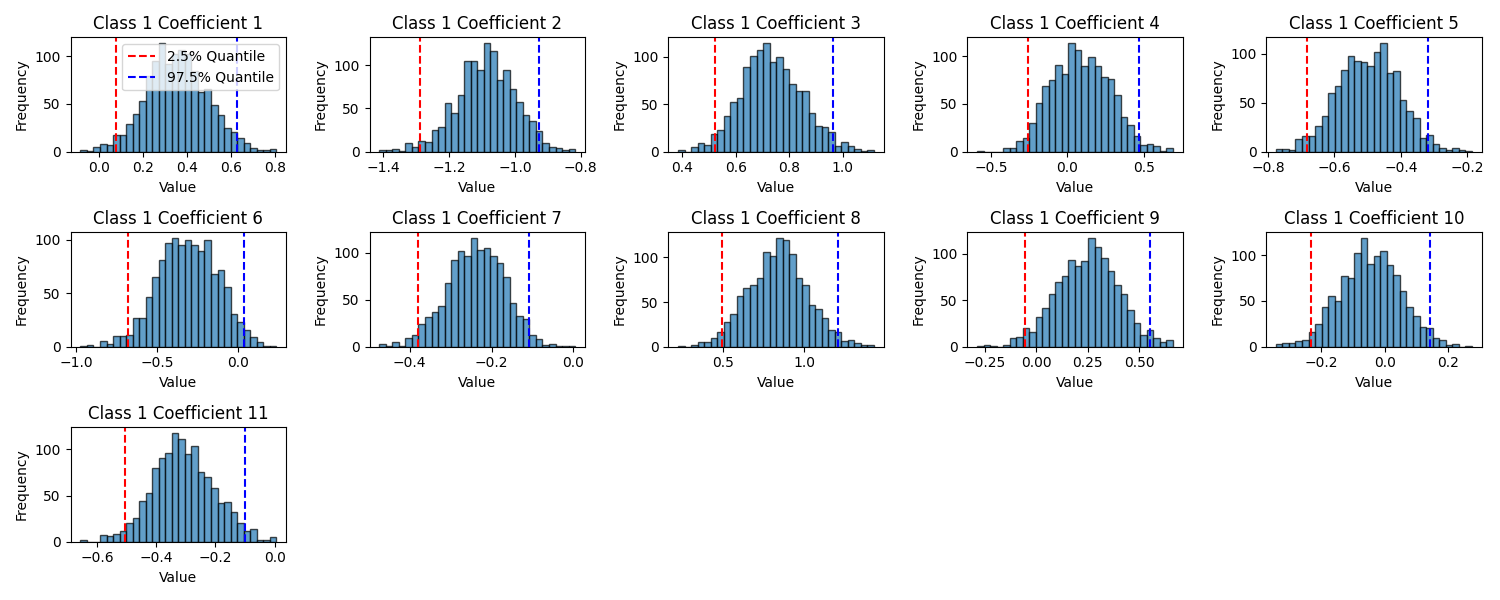
\includegraphics[width=1\textwidth]{../results/ModelFitting2/bootstrap_estimates_histograms.png}
    \caption{Bootstrap estimates histograms for prior distribution of $\beta_i$}
    \label{fig:bootstrap_estimates_histograms}
\end{figure}

Figure~\ref{fig:bootstrap_estimates_histograms}
\footnote{Here we only use class 1 in response variable to demonstrate how we obtain the distribution of 
$\beta_i$ from bootstrap method, that's there is 'Class 1' string in titles.} 
shows the empirical prior distributions of the
logistic regression coefficients $\beta_i$ estimated using bootstrap
resampling for class label 1 among the five target categories.
Each subplot corresponds to a coefficient in the model, including the intercept term. 

The histograms represent the frequency distribution of coefficient estimates across 
bootstrap samples, giving an approximation of the sampling distribution under repeated sampling. 
Vertical dashed lines mark the 2.5\% and 97.5\% quantiles, providing a 95\% empirical confidence 
interval for each $\beta_i$. These intervals reflect the uncertainty of the coefficients prior 
to incorporating the likelihood in the Bayesian inference step.

\begin{figure}[!h]
    \centering
    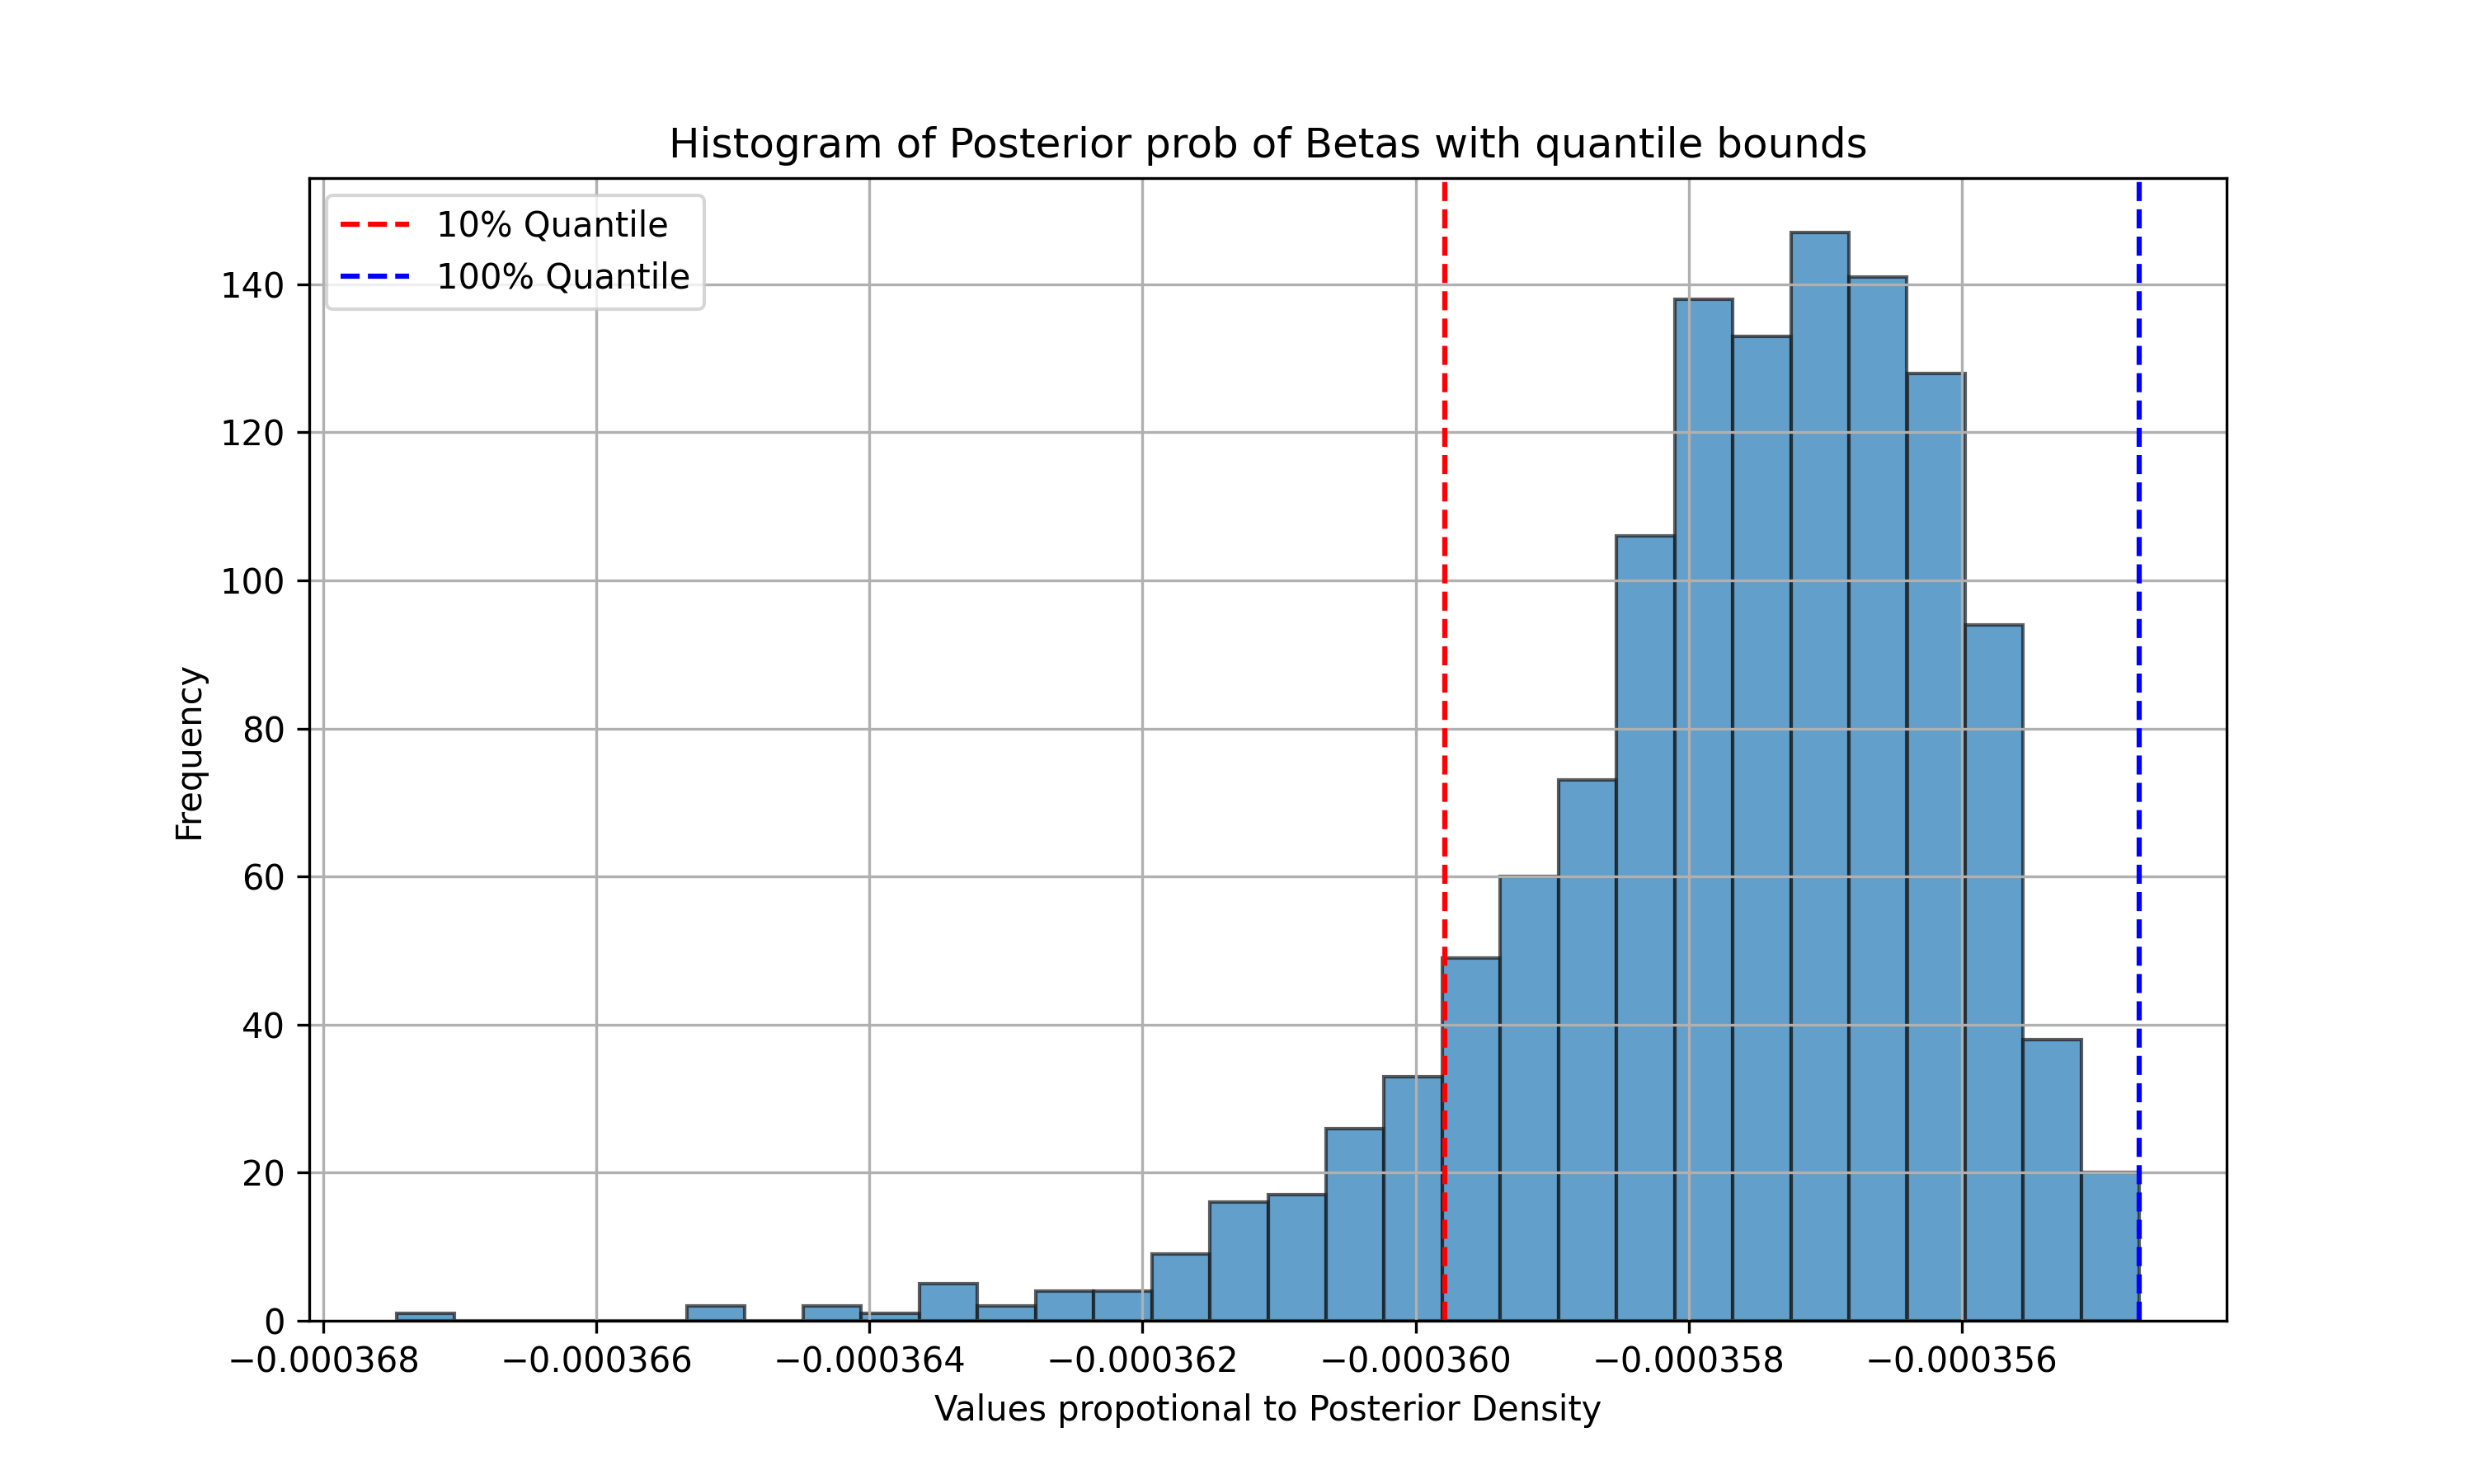
\includegraphics[width=0.9\textwidth]{../results/ModelFitting2/bayesian_posterior_density_histogram.png}
    \caption{Hist of values proportional to the posterior distribution of $\beta$ vector}
    \label{fig:bayesian_posterior_density_histogram}
\end{figure}

Figure~\ref{fig:bayesian_posterior_density_histogram} shows the histogram of values proportional to the posterior distribution of the logistic regression coefficients $\beta$. These values represent the product of the likelihood and the bootstrap-estimated prior, up to a normalization constant.

The vertical dashed lines indicate the 10\% and 100\% quantile thresholds, 
highlighting the top 90\% of posterior-proportional values. 
This range identifies the most probable $\beta$ candidates,
 useful for summarizing the posterior or computing the expected $\beta$
 \footnote{The computation is also based on class 1 among the 5 classes.}.

\subsection{Model performance evaluation}

After repeatedly training the model on 5 different classes, we can get the 
model performance metrics of the models.

Table ~\ref{tab:metrics_train} shows the model performance metrics of the performance of bayesian logsistic regression  
and MLE logistic regression model on training data.

\begin{table}[!h]
    \centering
    \caption{Model evaluation metrics grouped by target}
    \label{tab:metrics_train}
    \begin{tabular}{cccccc}
    \toprule
    \textbf{Target} & \textbf{Accuracy} & \textbf{Precision} & \textbf{Recall} & \textbf{F1 Score} & \textbf{Model} \\
    \midrule
    \multirow{2}{*}{1} & 0.8629 & 0.6111 & 0.8800 & 0.7213 & MLE \\
                       & 0.8629 & 0.6111 & 0.8800 & 0.7213 & Bayesian \\
    \midrule
    \multirow{2}{*}{2} & 0.6774 & 0.3729 & 0.8800 & 0.5238 & MLE \\
                       & 0.7016 & 0.3889 & 0.8400 & 0.5316 & Bayesian \\
    \midrule
    \multirow{2}{*}{3} & 0.6694 & 0.3095 & 0.5200 & 0.3881 & MLE \\
                       & 0.6855 & 0.3158 & 0.4800 & 0.3810 & Bayesian \\
    \midrule
    \multirow{2}{*}{4} & 0.6048 & 0.2549 & 0.5417 & 0.3467 & MLE \\
                       & 0.6774 & 0.3095 & 0.5417 & 0.3939 & Bayesian \\
    \midrule
    \multirow{2}{*}{5} & 0.7097 & 0.4000 & 0.8800 & 0.5500 & MLE \\
                       & 0.7419 & 0.4186 & 0.7200 & 0.5294 & Bayesian \\
    \bottomrule
    \end{tabular}
\end{table}

Table~\ref{tab:metrics_train} compares the performance of MLE and Bayesian logistic 
regression models on the training dataset across five target classes using standard 
classification metrics. Overall, both models exhibit consistent performance on class 1,
 achieving high accuracy (0.8629), precision (0.6111), recall (0.8800), and F1 score (0.7213),
  suggesting this class is well modeled.

For the remaining classes, Bayesian models tend to slightly outperform MLE models
 in terms of accuracy, precision, and F1 score. For example, in class 2, the Bayesian 
 model achieves higher accuracy (0.7016 vs.\ 0.6774) and better F1 score (0.5316 vs.\ 0.5238),
  despite both models showing strong recall (above 0.84).
   This trend continues in classes 3 and 4, where the Bayesian model improves
    on accuracy and precision, although the recall values remain close.
     Class 4 shows a notable improvement in accuracy (0.6774 vs.\ 0.6048) 
     and F1 score (0.3939 vs.\ 0.3467) for the Bayesian model.

In class 5, the Bayesian model again achieves higher accuracy (0.7419 vs.\ 0.7097), 
although its recall drops slightly compared to MLE (0.7200 vs.\ 0.8800), leading to a
 marginally lower F1 score. Overall, the Bayesian approach generally improves model 
 robustness across imbalanced classes by balancing precision and recall more effectively, 
 as reflected in consistently stronger F1 scores in most classes.


 \begin{table}[!h]
    \centering
    \caption{Model evaluation metrics on test data}
    \label{tab:metrics_test}
    \begin{tabular}{cccccc}
    \toprule
    \textbf{Target} & \textbf{Accuracy} & \textbf{Precision} & \textbf{Recall} & \textbf{F1 Score} & \textbf{Model} \\
    \midrule
    \multirow{2}{*}{1} & 0.5887 & 0.1389 & 0.2000 & 0.1639 & MLE \\
                       & 0.5887 & 0.1389 & 0.2000 & 0.1639 & Bayesian \\
    \midrule
    \multirow{2}{*}{2} & 0.4839 & 0.1695 & 0.4000 & 0.2381 & MLE \\
                       & 0.5081 & 0.1897 & 0.4400 & 0.2651 & Bayesian \\
    \midrule
    \multirow{2}{*}{3} & 0.5403 & 0.1190 & 0.2000 & 0.1493 & MLE \\
                       & 0.5645 & 0.1081 & 0.1600 & 0.1290 & Bayesian \\
    \midrule
    \multirow{2}{*}{4} & 0.5565 & 0.1961 & 0.4167 & 0.2667 & MLE \\
                       & 0.5968 & 0.1905 & 0.3333 & 0.2424 & Bayesian \\
    \midrule
    \multirow{2}{*}{5} & 0.4516 & 0.1091 & 0.2400 & 0.1500 & MLE \\
                       & 0.5323 & 0.1333 & 0.2400 & 0.1714 & Bayesian \\
    \bottomrule
    \end{tabular}
\end{table}

The evaluation on test data reveals a noticeable drop in performance for both models across 
all metrics. Accuracy ranges from approximately 45\% to 59\%, and F1 scores remain low,
 mostly under 0.27. This indicates challenges in generalizing beyond the training data. 
 Despite the overall low performance, the Bayesian model generally achieves slightly 
 higher F1 scores than MLE, particularly for targets 2, 4, and 5,
 suggesting better balance between precision and recall under uncertainty.


\begin{figure}[!h]
    \centering
    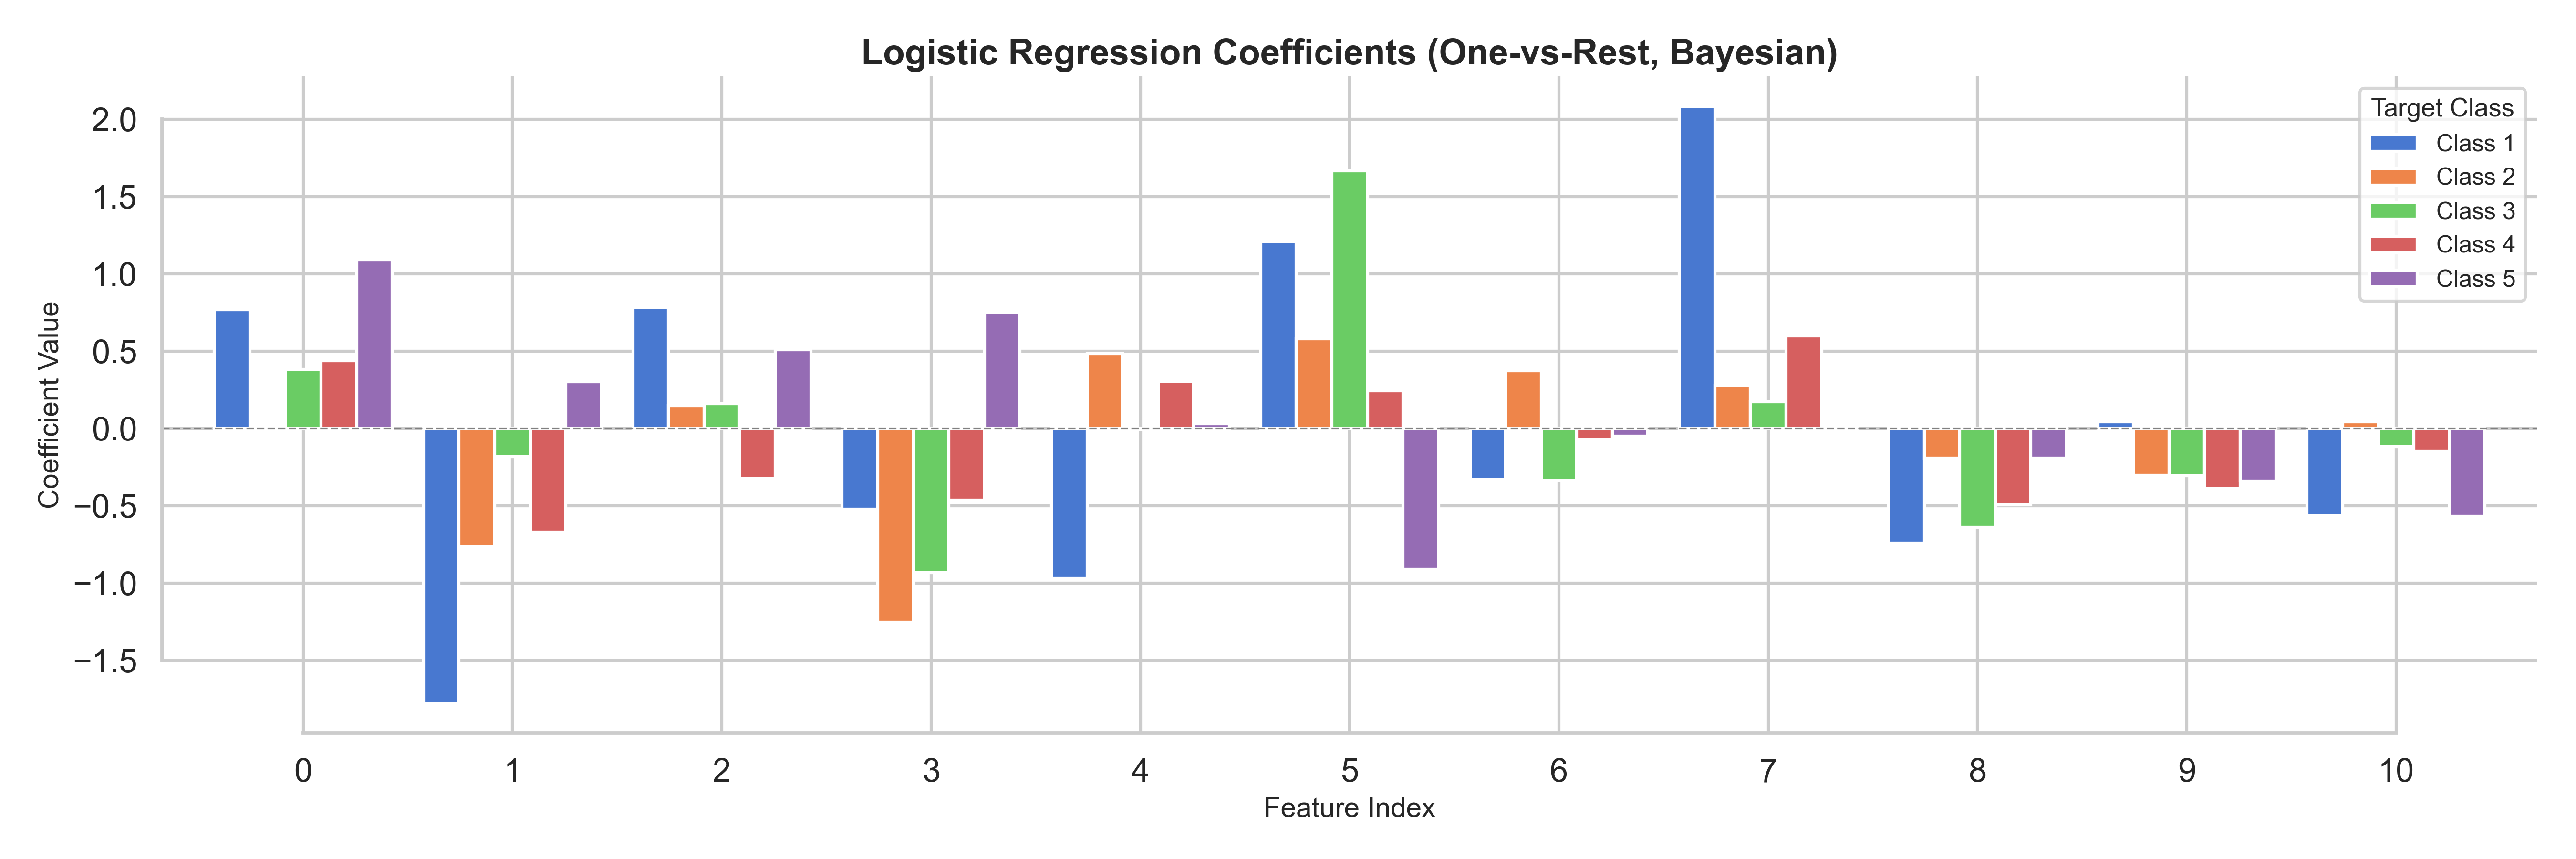
\includegraphics[width=0.9\textwidth]{../results/ModelFitting2/bayesian_coef_plot.png}
    \caption{The importance of each feature in the Bayesian logistic regression model}
    \label{fig:bayesian_coef_plot}
\end{figure}

Figure~\ref{fig:bayesian_coef_plot} illustrates the coefficients 
from five one-vs-rest Bayesian logistic regression models, each targeting a different class. 
Features with large absolute coefficient values have a stronger influence on the model's predictions.
 Notably, features indexed at 0, 1, 5, and 7 exhibit substantial variability across classes, 
 indicating their high discriminative power. For instance, feature 6 is particularly important
  for Class~1 and Class~4, while feature 5 plays a dominant role in Class~3. Conversely, 
  features 8--10 show relatively small coefficients across all classes, suggesting limited 
  influence on prediction. The direction (sign) of each coefficient also reveals whether a 
  feature increases or decreases the likelihood of the corresponding class.

\begin{figure}[!h]
    \centering
    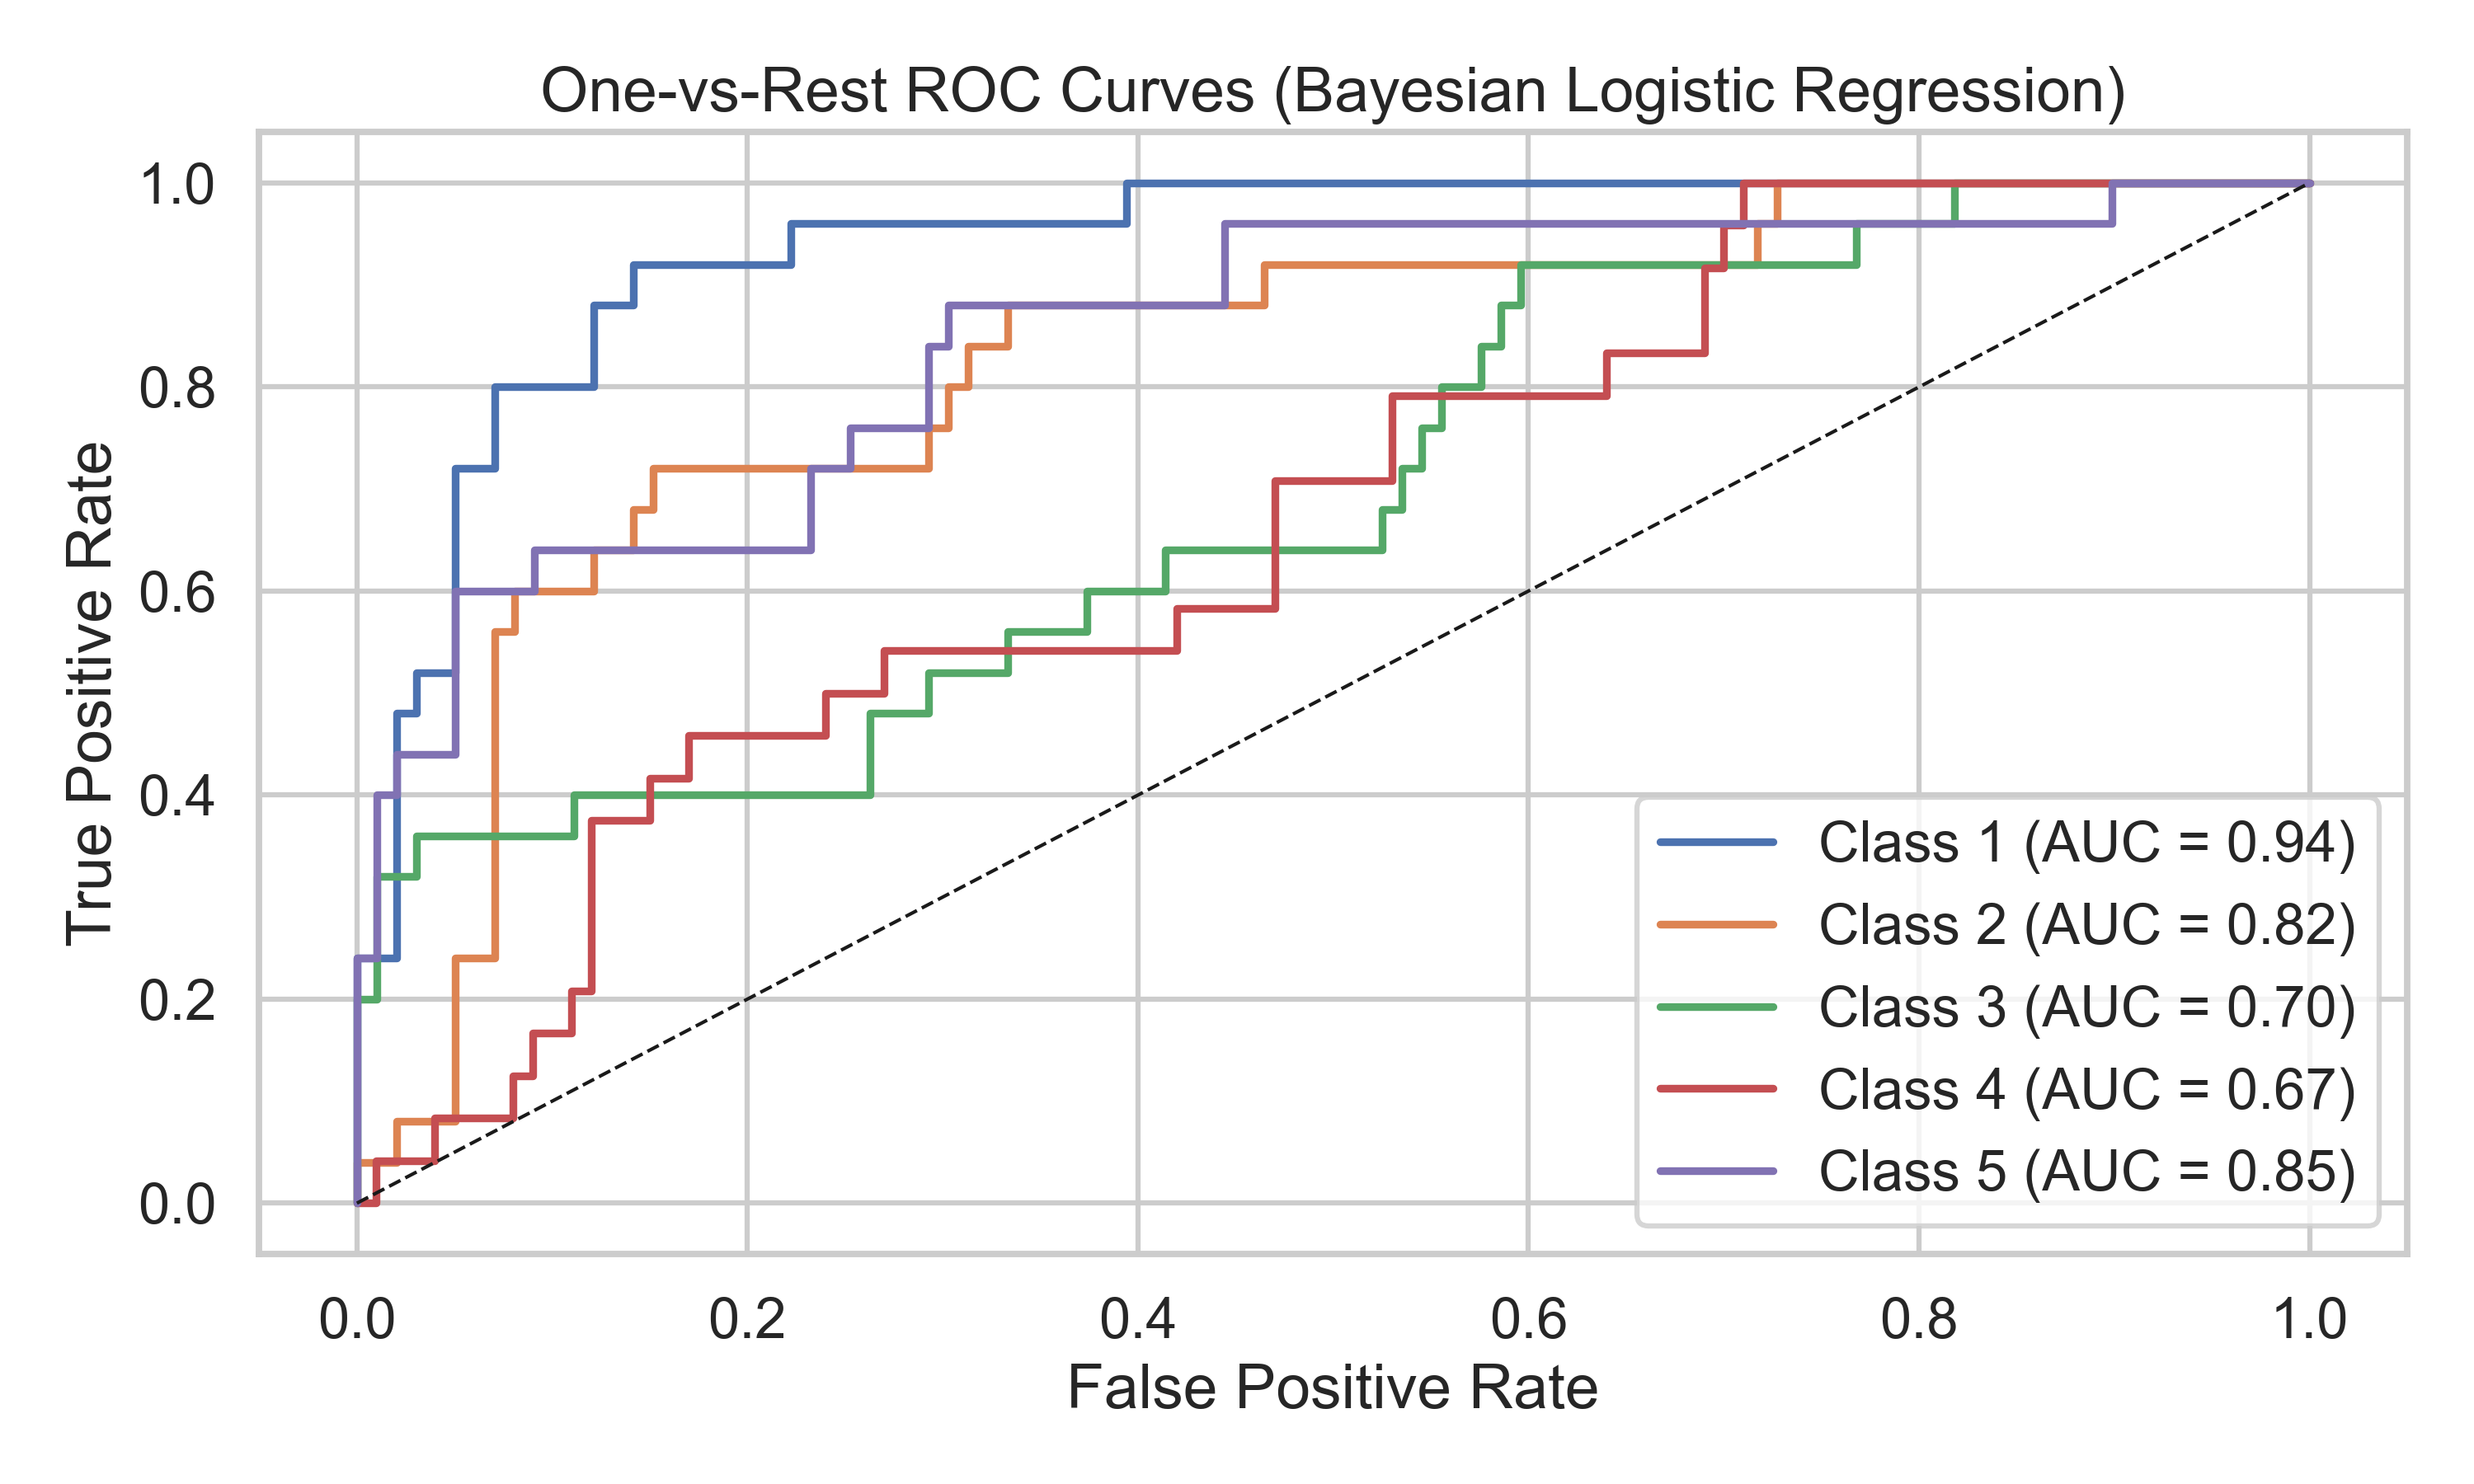
\includegraphics[width=0.9\textwidth]{../results/ModelFitting2/roc_curve_bayesian.png}
    \caption{ROC curve of each of the Bayesian logistic regression models across 5 classes}
    \label{fig:roc_curve_bayesian}
\end{figure}

Figure~\ref{fig:roc_curve_bayesian} displays the ROC curves for the five one-vs-rest Bayesian logistic regression models, each classifying one of the five target classes. 
The Area Under the Curve (AUC) serves as a summary of model performance, where higher values indicate better discrimination. Class~1 achieves the highest AUC (0.94),
 suggesting strong predictive performance. 
Class~5 and Class~2 also show good separation with AUCs of 0.85 and 0.82, respectively. In contrast, Class~3 (AUC = 0.70) and especially Class~4 (AUC = 0.67) demonstrate more 
limited classification ability, with curves closer to the diagonal, indicating greater confusion between classes. Overall, the ROC analysis highlights varying levels of model effectiveness across classes.